%==============================
\chapter{Results}\label{cap:resultado}
%==============================

This chapter presents the experimental results organized around the four research questions defined in Chapter~\ref{cha:methodology}. Section~\ref{sec:res_baseline} characterizes the sequential baselines. Section~\ref{sec:res_rq1} addresses RQ1 (correctness). Section~\ref{sec:res_rq2} addresses RQ2 (speedup). Section~\ref{sec:res_rq3} addresses RQ3 (failure characterization). Section~\ref{sec:res_rq4} addresses RQ4 (model comparison).

%==============================
\section{Sequential Baselines}
\label{sec:res_baseline}

Table~\ref{tab:baseline} reports the average execution time, standard deviation, Instructions Per Cycle (IPC), and cache miss rate for each sequential program over 30 runs. 
The measurements confirm stable execution times (standard deviation below 1\% of the mean in all cases) and reveal differences in computational character across programs.

\begin{table}[htbp]
\centering
\caption{Sequential baseline measurements (30 runs, \texttt{taskset} cores 1--11). IPC = instructions per cycle; Cache Miss = L1/LLC combined miss rate from \texttt{perf stat}.}
\label{tab:baseline}
\begin{tabular}{llrrrrr}
\toprule
%\textbf{Program} & \textbf{Complexity} & \textbf{Input ($N$} & \textbf{Avg Time (s)} & \textbf{Std Dev (s)} & \textbf{IPC} & \textbf{Cache Miss} \\
\textbf{Program} & \textbf{Complexity} & \textbf{Input} & \textbf{Time (s)} & \textbf{Std Dev (s)} & \textbf{IPC} & \textbf{Cache Miss} \\
\midrule
DP      & $O(N)$   & $10^{10}$ & 2.1686 & 0.0056 & 6.99 & 28.54\% \\
NI      & $O(N)$   & $10^{9}$  & 1.9774 & 0.0047 & 1.97 & 29.78\% \\
MM      & $O(N^3)$ & 2048      & 1.9369 & 0.0054 & 5.58 &  1.40\% \\
OE      & $O(N^2)$ & $10^{5}$  & 3.2849 & 0.0071 & 3.63 &  1.51\% \\
DFT     & $O(N^2)$ & $10^{4}$  & 1.7494 & 0.0103 & 3.02 &  1.44\% \\
TR      & $O(N^3)$ & 1280      & 1.8975 & 0.0155 & 5.20 & 39.37\% \\
\bottomrule
\end{tabular}
\fonte{The author.}
\end{table}

DP achieves the highest IPC (6.99), indicating that the processor efficiently pipelines the dot product accumulation with few stalls. Despite this, the cache miss rate of 28.54\% reflects the memory-bound nature of iterating over $10^{10}$ elements: the working set far exceeds all cache levels, and sequential accesses are serviced primarily from DRAM. NI presents a similar memory profile (29.78\% miss rate) but lower IPC (1.97), consistent with its dependence on floating-point transcendental functions such as cosine, which introduce pipeline stalls.

MM shows a very low cache miss rate (1.40\%) because the blocked matrix-multiplication access pattern keeps data in cache during the inner loop, enabling high IPC (5.58). 
OE and DFT also show low cache miss rates, consistent with their vector-based working sets fitting within the cache. 
TR exhibits the highest cache miss rate (39.37\%), reflecting frequent irregular accesses to the two-dimensional grid as the wavefront sweeps across diagonals.

%==============================
\section{RQ1: Correctness}
\label{sec:res_rq1}

\textbf{All 30 generated programs (5 models $\times$ 6 programs) compiled without errors and produced output identical to the sequential oracle.} Table~\ref{tab:correctness} records the correctness results.

\begin{table}[htbp]
\centering
\caption{Correctness: Output of each parallel version compared against the sequential oracle. \checkmark~= exact output match. All 30 programs compiled without errors.}
\label{tab:correctness}
\begin{tabular}{lrrrrr}
\toprule
\textbf{Program} & \textbf{ChatGPT} & \textbf{Gemini} & \textbf{Claude} & \textbf{Meta AI} & \textbf{DeepSeek} \\
\midrule
Dot Product           & \checkmark & \checkmark & \checkmark & \checkmark & \checkmark \\
Numerical Integration & \checkmark & \checkmark & \checkmark & \checkmark & \checkmark \\
Matrix Multiplication & \checkmark & \checkmark & \checkmark & \checkmark & \checkmark \\
Odd-Even Sort         & \checkmark & \checkmark & \checkmark & \checkmark & \checkmark \\
DFT                   & \checkmark & \checkmark & \checkmark & \checkmark & \checkmark \\
Turing Ring           & \checkmark & \checkmark & \checkmark & \checkmark & \checkmark \\
\bottomrule
\end{tabular}
\fonte{The author.}
\end{table}

The 100\% compilation and correctness rate is a notable finding. 
The programs evaluated extend from simple $O(N)$ reductions to $O(N^3)$ algorithms with complex data dependencies. 
Yet no model produced code that failed to compile or to produce numerically incorrect output. 
This result suggests that the five evaluated models have sufficient understanding of C syntax, the OpenMP programming model, and the algorithmic structure of the benchmark programs to produce functionally correct parallel implementations in a single attempt.

%==============================
\section{RQ2: Speedup}
\label{sec:res_rq2}

Table~\ref{tab:speedup} reports the speedup achieved by each LLM-generated program at 11 threads, together with the speedup achieved by the expert-written PAMPAR reference parallel implementation for each program.

\begin{table}[htbp]
\centering
\caption{Speedup $S = T_{\text{seq}} / T_{\text{par}}$ at 11 threads (30 runs each). 
$^\dagger$Meta AI NI: \texttt{\#pragma omp ordered} serializes the accumulation loop (see Section~\ref{sec:res_rq3}). 
$^\ddagger$DeepSeek TR: wavefront restructuring reduces iteration count from $O(N^3)$ to $O(N^2)$; the speedup reflects an algorithmic optimization and is excluded from the average (see Section~\ref{sec:res_rq3}).} 
\label{tab:speedup}
\begin{tabular}{lrrrrrr}
\toprule
\textbf{Program} & \textbf{Reference} & \textbf{ChatGPT} & \textbf{Gemini} & \textbf{Claude} & \textbf{Meta AI} & \textbf{DeepSeek} \\
\midrule
DP  & 4.59 & 5.37 & 5.42 & 5.43 & 5.39 & 5.35 \\
NI  & 5.35 & 5.26 & 5.27 & 5.26 & 0.48$^\dagger$ & 5.34 \\
MM  & 4.71 & 2.76 & 4.64 & 4.82 & 4.76 & 4.63 \\
OE  & 4.76 & 4.43 & 4.44 & 4.33 & 4.43 & 4.43 \\
DFT & 6.15 & 6.10 & 6.08 & 6.02 & 6.02 & 5.99 \\
\midrule
%\textbf{Average (excl.\ TR)} &
\textbf{Average} &
\textbf{5.11} & \textbf{4.79} & \textbf{5.17} & \textbf{5.17} & \textbf{4.22} & \textbf{5.15} \\
\midrule
TR  & 5.01 & 2.15 & 4.97 & 4.92 & 2.22 & 34.75$^\ddagger$ \\
\bottomrule
\end{tabular}
\fonte{The author.}
\end{table}

\textbf{Dot Product (DP).} All five LLMs exceeded the reference speedup of 4.59$\times$, achieving 5.35--5.43$\times$. The LLMs uniformly adopted a \texttt{reduction(+:)} clause over the dot product accumulation loop, which is the standard optimal OpenMP approach for this pattern. The reference implementation may use a different reduction strategy that is slightly less efficient under the measured conditions.

\textbf{Numerical Integration (NI).} Four of the five models achieved speedups of 5.26--5.34$\times$, close to the reference of 5.35$\times$. Meta AI achieved only 0.48$\times$, a slowdown relative to the sequential baseline. This failure is analyzed in Section~\ref{sec:res_rq3}.

\textbf{Matrix Multiplication (MM).} Gemini, Claude, and Meta AI achieved speedups of 4.63--4.82$\times$, matching or slightly exceeding the reference of 4.71$\times$. ChatGPT achieved only 2.76$\times$, a significant shortfall relative to both the reference and the other models. Analysis of the ChatGPT implementation revealed the same loop structure and data layout as the other models, but, definitively, no single cause for the performance gap was identified. DeepSeek achieved 4.63$\times$.

\textbf{Odd-Even Sort (OE).} All models achieved 4.33--4.44$\times$, slightly below the reference of 4.76$\times$. 
The OE sort alternates between odd and even phases.
Each requires a global synchronization barrier before the next phase begins. 
The slight gap relative to the reference may reflect minor differences in barrier implementation or loop scheduling.

\textbf{Discrete Fourier Transform (DFT).} All models achieved 5.99--6.10$\times$, very close to the reference of 6.15$\times$. DFT is an embarrassingly parallel algorithm where each output frequency coefficient is computed independently, making the outer loop trivially parallelizable with a reduction clause. The uniformly high speedup across all models confirms this.

\textbf{Turing Ring (TR).} Results were highly variable: Gemini achieved 4.97$\times$ and Claude 4.92$\times$ (close to the reference 5.01$\times$), while ChatGPT achieved 2.15$\times$ and Meta AI 2.22$\times$. DeepSeek achieved 34.75$\times$. The wide range reflects three distinct parallelization strategies adopted across the five models, analyzed in Section~\ref{sec:res_rq3}.

Figure~\ref{fig:speedup_program} illustrates the speedup of each model across the five programs DP, NI, MM, OE, and DFT, together with the reference implementation. The figure makes the two main performance failures immediately visible: the sharp drop of Meta AI on NI and of ChatGPT on MM, in contrast to the otherwise uniform behaviour close to the reference on the remaining programs. Turing Ring is shown separately in Figure~\ref{fig:turing_ring} due to its outlier behaviour.

\begin{figure}[htbp]
\centering
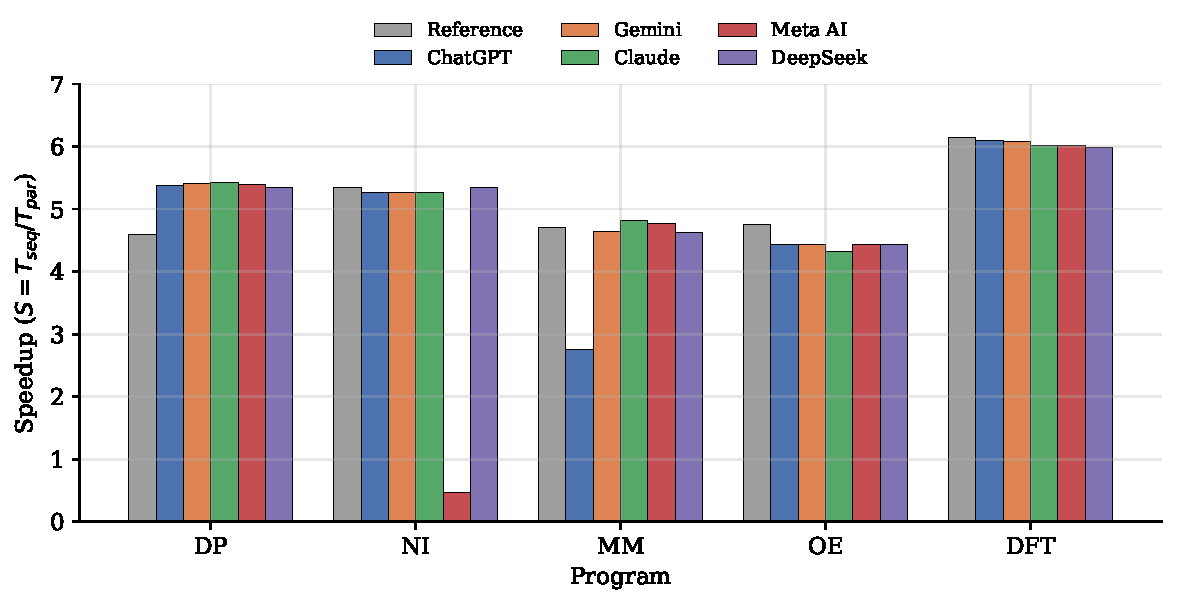
\includegraphics[width=\textwidth]{figuras/speedup_by_program.pdf}
\caption{Speedup per program at 11 threads for each LLM and the PAMPAR reference implementation. Turing Ring is shown separately in Figure~\ref{fig:turing_ring} due to its outlier behaviour.}
\label{fig:speedup_program}
\fonte{The author.}
\end{figure}

%==============================
\section{RQ3: Failure Characterization}
\label{sec:res_rq3}
%==============================

Two distinct classes of limitation were observed in the generated programs: a correctness-preserving performance failure (Meta AI NI) and a parallelization overhead problem (ChatGPT and Meta AI TR). Additionally, one case of an unexpected algorithmic optimization was observed (DeepSeek TR).

%==============================
\subsection{Meta AI Numerical Integration: \texttt{\#pragma omp ordered}}
\label{subsec:metaai_ni}

The Numerical Integration program computes the integral $\int_0^1 4/(1+x^2)\,dx$ using the rectangular rule with $N = 10^9$ sample points. Each iteration is independent: the value of the integrand at point $i$ depends only on $i$ itself and not on any previously computed value. The correct parallelization is a straightforward parallel reduction.

Meta AI's implementation placed a \texttt{\#pragma omp ordered} directive inside the parallel loop governing the accumulation of the partial sums:

\begin{verbatim}
#pragma omp parallel for ordered
for (long i = 0; i < N; i++) {
    double x = (i + 0.5) / N;
    double fx = 4.0 / (1.0 + x * x);
    #pragma omp ordered
    { total = total + fx; }
}
\end{verbatim}

The \texttt{ordered} clause forces each iteration of the loop to update \texttt{total} in the original sequential order, one thread at a time. 
That eliminates all parallelism in the accumulation, which is the dominant operation in this program. The code runs more slowly than the sequential version (speedup of 0.48$\times$) because it incurs thread management overhead on top of a full serialized computation. 
The output is numerically correct because the ordered execution preserves the original sequential order of additions.

The root cause of this failure is the model's decision to use \texttt{ordered} to avoid a race condition on \texttt{total}. While preventing the race condition, \texttt{ordered} is the wrong remedy: the correct solution is a \texttt{reduction(+:total)} clause, which maintains a private accumulator per thread and combines them at the end of the parallel region without any ordering constraint.

%==============================
\subsection{ChatGPT and Meta AI Turing Ring: Thread Spawn Overhead}
\label{subsec:chatgpt_metaai_tr}

The Turing Ring algorithm simulates a cellular automaton on a 1280$\times$1280 toroidal grid over multiple time steps. 
Parallelization requires recognizing a wavefront dependency: at each time step, cells along the same anti-diagonal of the grid are independent of others, but processing must proceed anti-diagonal by anti-diagonal in strict order.

The reference implementation and the implementations by Gemini and Claude correctly handle this structure by maintaining the outer anti-diagonal loop as serial and parallelizing only the inner loop over the cells within each anti-diagonal:

\begin{verbatim}
for (int d = 0; d < 2*N-1; d++) { //serial: one diagonal at a time
    #pragma omp parallel for schedule(dynamic)
    for (int i = start; i <= end; i++) { //parallel: cells on diagonal d
        joga(grid, i, d-i, N, aux);
    }
}
\end{verbatim}

ChatGPT and Meta AI adopted a structurally similar approach—parallel inner loop, like the serial anti-diagonal loop—but without processing the start and end bounds of each previous diagonal. 
As a result, their implementations iterate over all $N \times N$ cells in the inner loop for each of the $2N-1$ diagonals, relying on a runtime conditional to skip cells that do not belong to the current diagonal. 
That produces $O(N^3)$ inner-loop iterations in total (versus $O(N^2)$ for the bounded approach), and creates 2559 separate parallel regions (one per diagonal for $N=1280$), each incurring the cost of thread team creation and synchronization. 
The combined overhead of the unnecessary iterations and repeated thread spawning reduced the speedup to approximately 2.15$\times$ (ChatGPT) and 2.22$\times$ (Meta AI).

%==============================
\subsection{DeepSeek Turing Ring: Algorithmic Optimization}
\label{subsec:deepseek_tr}

DeepSeek's implementation of the Turing Ring achieved a speedup of 34.75$\times$, which exceeds both the reference implementation (5.01$\times$) and the theoretical linear speedup for 11 threads. This result warrants careful interpretation.

Inspection of the DeepSeek code reveals that the model did not simply add OpenMP directives to the original algorithm. Instead, it restructured the wavefront loop to compute explicit bounds for each anti-diagonal, thereby restricting the inner parallel loop to only the cells that belong to the current diagonal:

\begin{verbatim}
for (int d = 0; d < 2*N-1; d++) {
    int start = (d < N) ? 0 : d - (N-1);
    int end   = (d < N) ? d : N-1;
    #pragma omp parallel for private(col) schedule(dynamic)
    for (int row = start; row <= end; row++) {
        col = d - row;
        joga(grid, row, col, N, aux);
    }
}
\end{verbatim}

This restructuring reduces the total number of cell evaluations from $O(N^3)$ (as in the original sequential implementation, which checks all $N^2$ cells for each of the $2N-1$ diagonals) to $O(N^2)$ (iterating only over valid cells). For $N=1280$, this eliminates approximately $N-1 = 1279$ redundant evaluations per diagonal step, yielding a combined effect of algorithmic speedup and parallel execution that far exceeds what parallelization alone could provide.

The output produced by DeepSeek's implementation is correct, as verified against the sequential oracle. The 34.75$\times$ speedup is therefore genuine in the sense that the program produces correct results faster, but it reflects a fundamental algorithmic improvement rather than parallelization performance alone. This case is excluded from the model average in Table~\ref{tab:speedup}.

Figure~\ref{fig:turing_ring} summarizes the Turing Ring speedups on a logarithmic scale, which is necessary to accommodate the DeepSeek result alongside the others. The figure shows the three tiers clearly: Gemini and Claude near the reference, ChatGPT and Meta AI below it due to thread-spawn overhead, and DeepSeek far above as a result of its algorithmic optimization.

\begin{figure}[htbp]
\centering
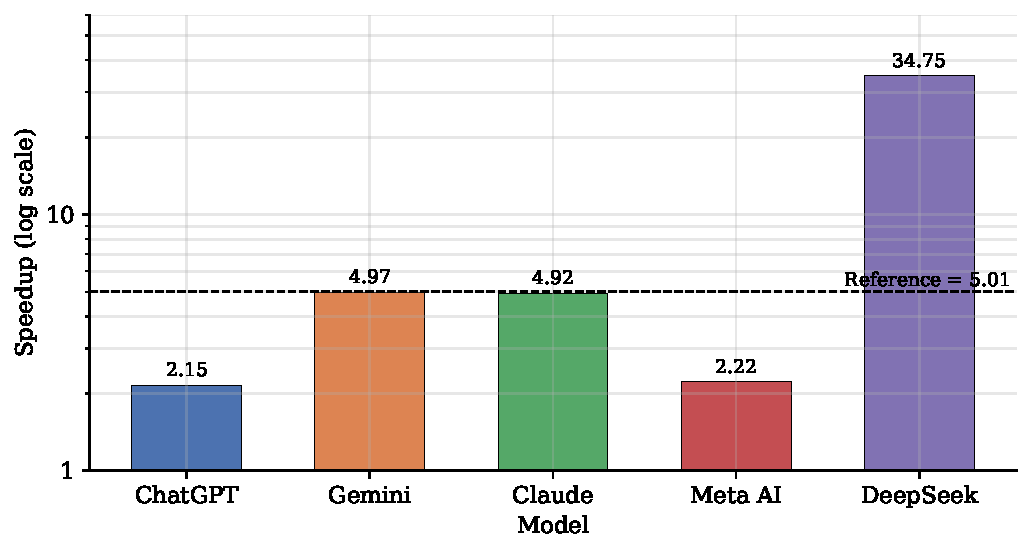
\includegraphics[width=.85\textwidth]{figuras/turing_ring_speedup.pdf}
\caption{Turing Ring speedup per model (logarithmic scale). DeepSeek's 34.75$\times$ reflects an algorithmic optimization rather than parallelism alone; ChatGPT and Meta AI fall below the reference due to thread-spawn overhead.}
\label{fig:turing_ring}
\fonte{The author.}
\end{figure}

%==============================
\section{RQ4: Model Comparison}
\label{sec:res_rq4}


All five models achieved 100\% compilation and correctness rates (RQ1). The primary differentiator is performance (RQ2).

The averages reported here are computed for the five programs DP, NI, MM, OE, and DFT, excluding Turing Ring (TR) for \emph{all} models, to compare the models on a basis.
TR is excluded uniformly because it concentrates effects that are not representative of directive-level parallelization: an algorithmic restructuring by DeepSeek and a thread-spawn overhead pattern in ChatGPT and Meta AI. TR is analyzed on its own in Section~\ref{sec:res_rq3}.

On this consistent basis, Gemini and Claude (both 5.17$\times$) most closely matched the PAMPAR reference implementation (5.11$\times$), with DeepSeek (5.15$\times$) essentially equivalent. ChatGPT (4.79$\times$) was lower, primarily driven by its suboptimal MM implementation (2.76$\times$). Meta AI performed the worst (4.22$\times$), driven by the severe NI failure (0.48$\times$). Including TR would not change this ordering for the four non-anomalous models, but would distort the DeepSeek average upward due to its algorithmic optimization.

On the simpler programs (DP, NI, DFT), all models performed comparably and close to the reference. Performance differences emerged only for programs with more complex parallelization requirements: MM (where ChatGPT's implementation underperformed), OE (where all models were marginally below the reference), and TR (which separated the models into three tiers based on parallelization strategy).

Figure~\ref{fig:avg_speedup} presents the average speedup per model on this consistent basis, making the overall ranking immediately apparent: Gemini, Claude, and DeepSeek cluster at the reference level, while ChatGPT and Meta AI trail behind due to their program-specific failures.

\begin{figure}[htbp]
\centering
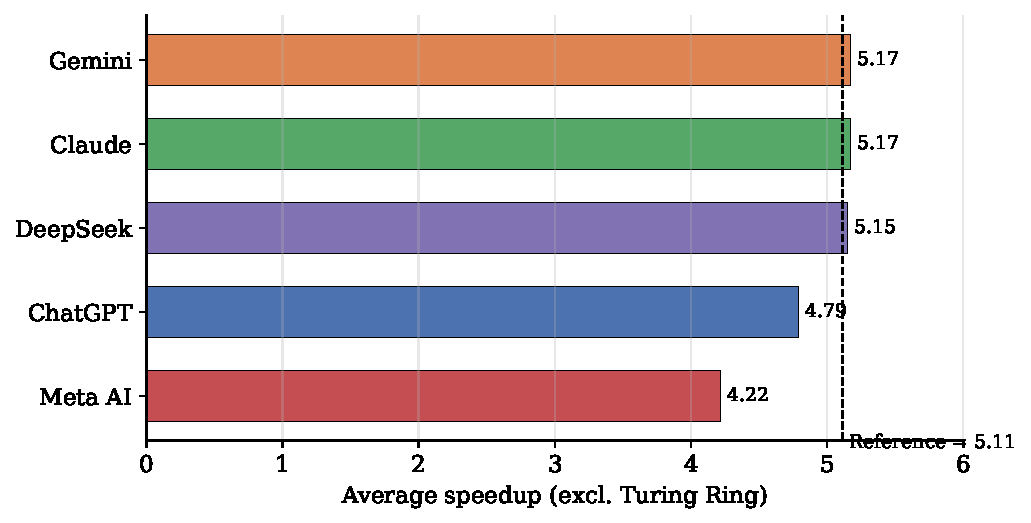
\includegraphics[width=.85\textwidth]{figuras/average_speedup.pdf}
\caption{Average speedup per model over DP, NI, MM, OE, and DFT (Turing Ring excluded uniformly). The dashed line marks the reference average.}
\label{fig:avg_speedup}
\fonte{The author.}
\end{figure}

Table~\ref{tab:model_summary} summarizes the comparative results.

\begin{table}[htbp]
\centering
\caption{Model summary: correctness rate, average speedup, and notable cases.}
\label{tab:model_summary}
\begin{tabular}{lccl}
\toprule
\textbf{Model} & \textbf{Correct (of 30)} & \textbf{Speedup} & \textbf{Notable case} \\
%\textbf{Model} & \textbf{Correct (of 30)} & \textbf{Avg Speedup} & \textbf{Notable case} \\
\midrule
%Reference (PAMPAR) & ---  & 5.11$\times$ & --- \\
Reference & ---  & 5.11$\times$ & --- \\
ChatGPT            & 6/6  & 4.79$\times$ & MM: 2.76$\times$; TR: overhead \\
Gemini             & 6/6  & 5.17$\times$ & TR: close to reference \\
Claude             & 6/6  & 5.17$\times$ & TR: close to reference \\
Meta AI            & 6/6  & 4.22$\times$ & NI: 0.48$\times$ (ordered failure); TR: overhead \\
DeepSeek           & 6/6  & 5.15$\times$ & TR: 34.75$\times$ (algorithmic) \\
\bottomrule
\end{tabular}
\fonte{The author.}
\end{table}

\noindent All averages are computed over DP, NI, MM, OE, and DFT (TR excluded uniformly); see Section~\ref{sec:res_rq3} for the TR analysis.